
%---------------------------------------------------------------
\chapter{The P4 Language}
%---------------------------------------------------------------

\begin{chapterabstract}
	\dots in which we delve into the syntax and semantics of \acrshort{p4},
	explain its use cases, and discuss the differences to conventional
	programming languages.

	\begin{displayquote}
		\textit{The expressive power of a programming language arises from its
		strictures and \emph{not} from its affordances.}

		-- Robert Harper, \citedate*{pfpl1oplss2019} \cite{pfpl1oplss2019}
	\end{displayquote}
\end{chapterabstract}

One of the original motivations behind \acrshort{p4} was the need for
restriction. While other \acrlong{dsl}s, such as Click\cite{kohler2000click},
existed at the time, their embeddings within general-purpose programming
languages made it difficult to analyze data dependencies crucial for scheduling
parallel execution. The expressiveness of a language complicates its efficient
compilation.

Rather than embedding \acrshort{p4} in an existing language, these
considerations motivated a clean-slate design. However, to understand why is
packet processing any different from tasks suited to general-purpose programming
languages, we first need to familiarise ourselves with the switching
architecture.

%----------------------------%
\section{What's in a switch}
%----------------------------%

\begin{displayquote}
	{[Packet switching is]} \emph{the routing and transferring of data by means
	of addressed packets so that a channel is occupied during the transmission
	of the packet only, and upon completion of the transmission the channel is
	made available for the transfer of other traffic.}

	-- \citetitle*{weik2012fiber} \cite{weik2012fiber}
\end{displayquote}

In the following text, we choose to use \emph{switch} to mean a general packet
switching device. Such a device could be a dedicated piece of hardware or a
software solution running on a general-purpose computer.

Traditionally, these devices were implemented by fixed-function hardware.
Various networking protocols were built directly into the circuitry, which made
these switches efficient, but inflexible. It is impossible to reconfigure a
fixed-function \acrfull{asic} to process a protocol it was not explicitly
designed for in advance. If a new, backward-incompatible version of a given
protocol emerges, or if a hardware error is found in the chip, the network
administrators need to perform a costly hardware replacement in order to support
or circumvent it, respectively. Moreover, fixed-function hardware design is a
lengthy and resource-intensive process. It may take several years before an
updated fixed-function chip hits the market.

The innovation of recent years is the introduction of \emph{programmable}
network processors, which can change the set of supported protocols on the fly.
These are similar to \acrshort{fpga}s in their reconfigurability, but
specialised to packet switching and routing, which makes them more efficient. A
programmable network switch has typically no prior knowledge of networking
protocols but contains efficient circuitry for parsing and pattern-matching in
order to support arbitrary\footnote{To some degree of complexity supported by
the circuit.} protocols uploaded to the chip as microcode. While programmable
networking hardware does incur a penalty for reconfigurability, when it comes to
efficiency, it sits between fixed-function devices and completely
general-purpose solutions.

Other implementations of packet switching are also common. The already mentioned
\acrlong{fpga}s can be programmed to simulate programmable or fixed-function
networking hardware, and thus allow an even higher degree of flexibility.
Naturally, \acrshort{fpga}s are less efficient than the circuits they simulate.
Finally, there are software switches, programs for widespread processor
architectures and operating systems, such as x86 and Linux. A software switch
represents the peak of flexibility, programmability, and requires no special
hardware other than what is already commonly present in conventional computers.
Purely software-based solutions cannot compete in energy efficiency with any of
the other approaches, but are often useful for testing and in small-scale
networks.

\begin{figure}[t]
	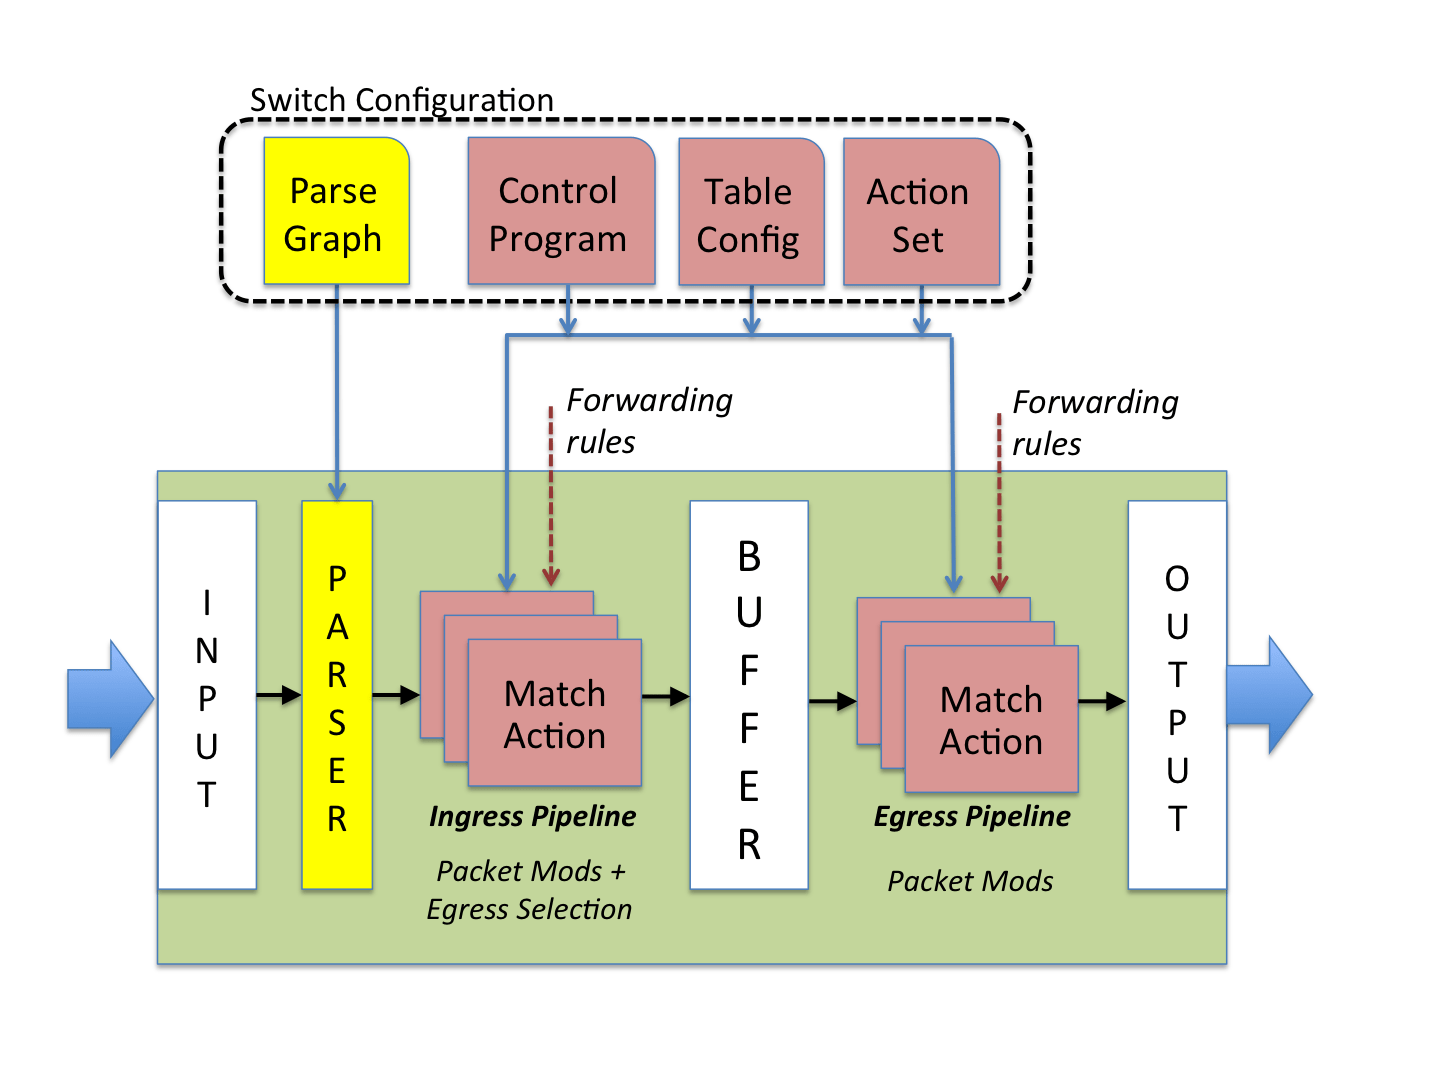
\includegraphics[
		trim={2.0cm 4.3cm 4.0cm 3.3cm}, % left bottom right top (insane, I know)
		width=1.00\textwidth
	]{resources/abstract-forwarding-model.png}
	\caption{The original \acrshort{p4}\textsubscript{14} abstract forwarding
	model, taken from \cite{p4original}.}
	\label{fig:abstract-forwarding-model}
\end{figure}

To support network configurations regardless of their physical implementation,
the original \acrshort{p4} paper defines the target-independent \emph{abstract
forwarding model}, outlined in Figure~\ref{fig:abstract-forwarding-model}. There
is a key conceptual split in the architecture, common in packet processing in
general, of the \emph{data plane} and the \emph{control plane}. We will meet
these terms over and over, so let us define them here.

\begin{description}
	\item[Data plane] is the part of the switch responsible for packet
	processing, i.e. all the hard work of manipulating bits in the arriving
	packets and choosing where to send the packets next. It is the part that is
	programmable in \acrshort{p4}, though it is unchanging in traditional packet
	processing approaches. The data plane is responsible for packet parsing,
	pattern-matching, and rewriting.
	\item[Control plane] is the part of the switch responsible for
	configuration. It is not programmable in \acrshort{p4}, but \acrshort{p4}
	programs implicitly define a software interface for it. The control plane is
	responsible for uploading forwarding rules to the data plane, extracting
	data from special fixed-function devices (such as throughput counters), and
	reconfiguring the flexible parts of the \acrshort{p4} program at runtime. A
	control plane program could be a simple Python script or a C++ application.
\end{description}

\subsubsection*{Parallels to general-purpose computing}

It is helpful to think of the data plane as an infrequently changing program
running on a network chip\footnote{Even though, as discussed, it could reside
entirely in software.}. It defines the protocols the switch can handle and the
stages of packet processing the switch performs, but not the concrete forwarding
rules, which can change at runtime.

In contrast, the control plane typically runs on a general-purpose computer and
uses the data plane as a coprocessor. It uploads forwarding rules (e.g. which
subnet to forward an arriving packet to) to coprocessor-specific memory. The
interface between the control plane and the data plane depends entirely on the
\acrshort{p4} program that the data plane runs, and relies on a hardware link
between the two, such as PCI Express.

The abstract forwarding model assumes an end-to-end data plane pipeline split
into \emph{ingress} and \emph{egress} parts. An arriving packet is first parsed
to recognize the headers present therein. These headers then travel through the
pipeline's \emph{match-action units}. Each match-action unit performs limited
pattern-matching and rewriting on the parsed packet header -- complex
\acrshort{p4} code can map to a sequence of several match-action units. This
part of the pipeline is partially configured at runtime by the control plane,
usually by forwarding rules defined in software.

To relate match-action units to conventional computing, they are similar to
cycles in a \acrshort{cpu} pipeline. In fact, the entire abstract forwarding
model can be thought of as the unrolling of a limited number of cycles of a
\acrshort{cpu} pipeline. This corresponds well to \acrshort{p4}'s lack of
looping constructs.

Packet headers (supplemental data placed at the beginning of a packet) are a
central concept in packet processing, and therefore also in the \acrshort{p4}
language. The abstract forwarding model assumes that the packet is split into
two parts: the header and the payload. Only the header proceeds into the
match-action pipeline\footnote{Although what part of the packet actually is
``the header'' is entirely up to the \acrshort{p4} program.}. The model assumes
that the payload is handled separately by the device and is thus not available
for pattern-matching.

\subsubsection*{Keeping it high-level}

While the presented forwarding model gives a good overview, it is not the full
picture. A notable omission is packet output. If the \acrshort{p4} program
implements a switch, how does the packet exit the pipeline? How does it select
the output port? And how does the switch filter out packets that should not be
forwarded?

These questions touch on the issue of supporting use-cases and functionality too
granular to be part of the abstract forwarding model. While they may seem like
blatant oversights, these omissions of packet processing details are deliberate.
\acrshort{p4} supports both output port selection and packet filtering via
packet \emph{metadata}. Intrinsic metadata is a target-dependent data structure
that stores information about a given packet and is available to the
\acrshort{p4} program at every stage of the pipeline, including parsing.
Metadata may include the input port and other information provided by the
device. Crucially, the metadata is typically mutable, and contains fields and
flags for the output port, recirculation, packet dropping, and other features.

The final stage of the processing pipeline in programmable network hardware
involves \emph{deparsing}, i.e. serializing the packet header back into a
bitstream. As we will see on page~\pageref{sec:p4-deparsing}, deparsing is a
case of a more general control mechanism that does not need special treatment
in the abstract model.

The design philosophy of reliance on general-purpose constructs, such as
metadata or \extern{}s (which we will see later), underpins much of the
\acrshort{p4} language, and its effects can be seen in many facets of the \pfs
revision. It makes the language both simpler, as it avoids accumulating narrow
use-case features, and more flexible, since it generalizes to platforms to which
these concepts do not translate.

%-----------------------%
\section{A tour of \pfs}
%-----------------------%

\begin{figure}[t]
	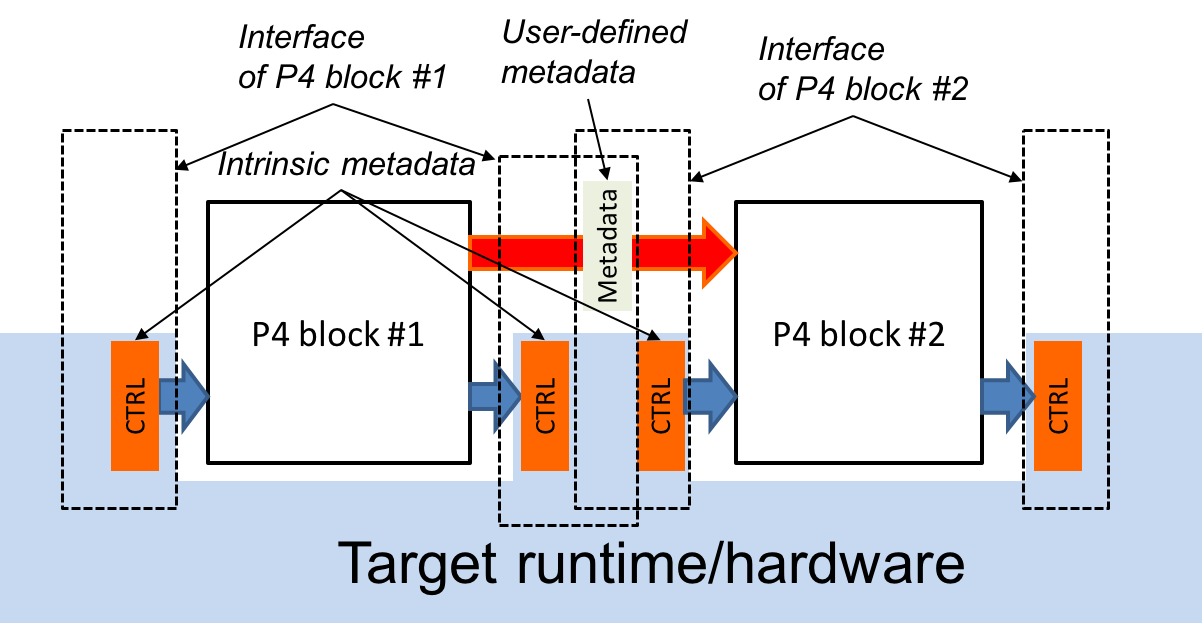
\includegraphics[width=1.00\textwidth]{resources/p4_16-architecture-model.png}

	\caption{\pfs program interfaces for an abstract architecture with two
	programmable blocks, taken from \cite{p416:v123:spec}.}
	\label{fig:arch-model}
\end{figure}

This section largely mirrors the \pfs language specification. It does not cover
the entire language, but should serve as a decent introduction to its most
important features, while attempting to draw some parallels to conventional
programming languages and terms of general-purpose computing.

A \acrshort{p4} program specifies a mapping of vectors of bits -- a bit\-vector
endomorphism. Every \acrshort{p4} program terminates; the language has no
looping constructs and no recursion, a compiler can thus determine the precise
maximum runtime of a program statically.

\acrshort{p4} is therefore not a programming language for von Neumann
architectures. Instead, its abstract model assumes the target machine to be some
sort of network processor with programmable blocks embedded in a static
pipeline. The overhaul into \pfs slightly redefined the abstract forwarding
model, as can be seen in Figure~\ref{fig:arch-model}. This diagram focuses on
the interfaces of the \acrshort{p4} program and points out metadata, which
deserves a special mention.

Practical implementations of \acrshort{p4}-configurable network hardware often
need to track information not included in the packet headers. This is especially
the case for devices with multiple pipelines, such as the one outlined in
Figure~\ref{fig:arch-model}, where the partial computation results from one
pipeline need to travel to the next in order to continue processing. The nature
of passing such metadata is heavily target-dependent, however. Some
architectures may include explicit side-channels for metadata and reflect this
in the interfaces they provide to user code, while other targets demand that the
user includes metadata explicitly in the packet headers. In other words, the
user metadata channel in P4\textsubscript{16}'s abstract forwarding model is
purely conceptual.

\todo[inline]{in discussing the subpar nature of the spec, include examples of
	mistakes.
	\href{https://p4.org/p4-spec/docs/P4-16-v-1.2.3.html\#sec-minsizeinbits}
	{compile-time size determination} mentions ``\emph{Each of these method
	calls evaluate to compile-time known values that return the minimum size in
	bits required to store the expression,}'' clearly forgetting to take the
	\texttt{maxSize*} functions into account}

\subsection{Syntax and semantics}

\todo[inline]{
	describe headers and their relation to structs, explain annotations
}

% relevant p4 spec sections

% 6.1.   Syntax and semantics
% 6.1.1. Grammar
% 6.1.2. Semantics and the P4 abstract machines
% 6.2.   Preprocessing
% 6.2.1. P4 core library
% 6.3.   Lexical constructs
% 6.3.1. Identifiers
% 6.3.2. Comments
% 6.3.3. Literal constants
% 6.4.   Naming conventions
% 6.5.   P4 programs
% 6.5.1. Scopes
% 6.5.2. Stateful elements
% 6.6.   L-values
% 6.7.   Calling convention: call by copy in/copy out
% 6.7.1. Justification
% 6.7.2. Optional parameters
% 6.8.   Name resolution
% 6.9.   Visibility

\pfs syntax is reminiscent of imperative programming languages in the C family.
It uses prefix notation for typed bindings, braces for lexical scoping blocks,
and semicolons to separate statements. However, instead of functions or
procedures, the dominant top level constructs for executable code are control
blocks and parsers, neither of which has a close relative in the world of conventional general-purpose computing.

The semantics of \pfs is defined entirely in terms of abstract machines
executing imperative code. A conforming compiler is free to rewrite the \pfs
program as long as it maintains the observable behaviour of all abstract
machines involved. Unfortunately, the specification gives no formal treatment
of these machines; they are described only in natural language and pseudocode.

The authors of the specification acknowledge that undefined behaviour has been
the cause of many problems in conventional languages and deliberately try to
avoid it. However, several constructs in the language are still underspecified
and users may run into undefined behaviour, for example by accessing the field
of an invalid header.

\subsection*{Imports and the core library}

Although not a language construct in its own right, the \acrshort{p4} core
library is a set of common programming definitions distributed together with
language tooling. Unlike preludes in certain programming languages, the core
library is not automatically included in every \acrshort{p4} program and must be
imported explicitly with the preprocessor directive \texttt{\#include
<core.p4>}. \pfs does not have a module system and relies solely on the C
preprocessor (or a sufficiently capable subset thereof) for code reuse.

\subsection*{\extern{} objects and functions}

Before diving into the bulk of the syntactical forms that dominate user-written
\acrshort{p4} code, we need to introduce the general concept of \extern{}s.

\extern{} objects and functions describe interfaces to facilities provided by
the architecture, as well as certain built-in language constructs\footnote{Such
as the \texttt{packet\_in} intrinsic in Listing~\ref{lst:p4-prsr-packet-in}}.
For example, the \extern{} object in Listing~\ref{lst:p4-extern-cksum} allows
\acrshort{p4} code to utilize a fixed-function checksum unit provided by the
target. The object specifies no implementation for the listed constructors and
methods, rather, the target platform implements the asserted functionality
intrinsically, e.g. by fixed-function circuitry.

To invoke a method of the checksum unit, the user needs first to
\emph{instantiate} the \extern{} object. This syntactic form is shared among all
types with constructors: \texttt{control} blocks, \texttt{parser}s, and
\texttt{package}s\todo{describe those somewhere}. The effect of an instantiation
is to allocate the corresponding object, binding it to the specified name.

The compiler is in charge of mapping instances of \extern{}s to the target
architecture (i.e. performing the allocation of resources on the target). If it
does not find a mapping, either because the target does not support the
\extern{} or does not have the resources to fit all its instances, the
compilation fails with an error.

\extern{} objects and functions were already present in
\acrshort{p4}\textsubscript{14} version 1.1, but \pfs fully embraced these
constructs. This helped to both simplify and generalize the language and led to
the elimination of several less general concepts. For example,
\acrshort{p4}\textsubscript{14} had dedicated syntax for checksum units.

\begin{lstlisting}[
	caption={~An \extern{} object specifying
	the interface to the target's checksum unit.},
	label=lst:p4-extern-cksum,
	captionpos=t,
	tabsize=4,
	float,
	abovecaptionskip=-\medskipamount,
	belowcaptionskip=\medskipamount,
	language=p4
]
extern Checksum16 {
	Checksum16();              // constructor
	void clear();              // prepare unit for computation
	void update<T>(in T data); // add data to checksum
	void remove<T>(in T data); // remove data from existing checksum
	bit<16> get(); // get the checksum for the data added since last clear
}
\end{lstlisting}

\subsection*{l-values}

\pfs has a concept of \emph{l-values}, reminiscent of C. An l-value is an
expression that denotes a memory cell that can be assigned to. These include

\begin{itemize}
	\item variables; identifiers of a base or derived type\todo{derived type!},
	\item fields of structs, headers, and header unions, and
	\item the results of bit-slice operators (e.g. \texttt{pkt[0:7]}).
\end{itemize}

\subsection*{Annotations}

\begin{lstlisting}[
	caption={~A structured annotation on a table.},
	label=lst:p4-annotation,
	captionpos=t,
	tabsize=4,
	float,
	abovecaptionskip=-\medskipamount,
	belowcaptionskip=\medskipamount,
	language=p4
]
@MyAnnotation[1, 2, 3]
table myTable { /* ... */ }
\end{lstlisting}

Almost all syntactical constructs in \pfs can be modified by \emph{annotations}
(see Listing~\ref{lst:p4-annotation}). These come in two flavours, structured
and unstructured, depending on the restrictions imposed on their arguments.
Unstructured annotations can take arbitrary token streams as their arguments, so
long as the parentheses in these token streams are balanced.

Very few annotations are built into the language, so we will not discuss them in
depth, but they provide an important avenue for target-specific extension of the
language.

\subsection*{Functions and parametrized code}

Functions in \acrshort{p4} come in several flavours. The first kind is known as
\emph{function declarations} and is perhaps the closest relative of procedures
in conventional imperative programming languages. The major difference is that
all parameters to a \acrshort{p4} function need to include a \emph{direction}.

\begin{description}
	\item[parameter direction] is either \texttt{in}, \texttt{out}, or
	\texttt{inout}. \texttt{in} indicates a read-only parameter with a defined
	value, \texttt{out} indicates a read-write parameter whose value is
	initially undefined upon entering the function body, and \texttt{inout}
	indicates a read-write parameter with a defined value.
\end{description}

Only l-values can be passed as \texttt{out} and \texttt{inout} parameters. The
execution of the function call can change the value of an \texttt{out} or
\texttt{inout} parameter's corresponding l-value. Note that \acrshort{p4}
functions can combine \texttt{out} parameters and return values.

Parameter directions are \acrshort{p4}'s way of introducing a limited form of
references, themselves a principled approach to pointers. Parametrized
\acrshort{p4} code follows a copy in / copy out calling convention, which makes
functions easy to reason about and limits side effecting behaviour of \extern{}
methods. We will discuss this later in ?\todo{reference here}

\subsection*{Parsers}

Another construct for parametrized code are \emph{parser declarations}. A
\acrshort{p4} parser describes a \acrlong{fsm} whose job is to recognize valid
packets and load their headers into the storage facilities of the target. Parser
declarations define all the states of the \acrshort{fsm}, except the implicit
built-in \texttt{accept} and \texttt{reject} states further described in the
semantics section\todo{reference here}. Each parser has to contain at least the
initial \texttt{start} state. During parsing, the parser can manipulate local
state\todo{context?} in the form of variables and \extern{} instantiations.
These are defined directly in the parser declaration block, before listing any
states, meaning that the type of this local context is statically known and
independent of the state the parser may appear in at runtime. In other words,
parser declarations follow lexical scoping.

States can introduce lexically-scoped local variables, but not additional
\extern{}s. Other statements like conditionals, assignments, or method calls are
also allowed. The specification explicitly points out that specific target
architectures can place restrictions on the set of constructs and operations a
programmer can use within a parser.

\pfs parser declarations unrestricted by the target architecture may appear very
similar to conventional imperative code, and reminiscent of other function-like
constructs the language offers. The crucial parser-only features are data
extraction, pattern-matching, error handling, and state transitions.

Data extraction moves information from the input packet into memory available
for pattern-matching further down the pipeline, typically registers or similar
containers. To facilitate this operation, the \acrshort{p4} core library
contains an intrinsic\footnote{By an ``intrinsic,'' we mean a language feature
that somehow invokes a mechanism native to the host architecture, one that could
not be defined in the language itself, or not as efficiently, and needs to be
hard-coded in the compiler.} \extern{} definition called \texttt{packet\_in}
which represents incoming packets. This special \extern{} cannot be manually
instantiated\todo{make sure we explain instantiation prior to this. Maybe
externs should be described first in the syntax section?}, but it is
instantiated implicitly for every parser parameter of type \texttt{packet\_in}.
This allows parser states to invoke the methods of the \extern{}, shown in
Listing~\ref{lst:p4-prsr-packet-in}.

\subsubsection*{Parser abstract machine}

A parser semantically manipulates a \texttt{ParserModel} data structure.

\begin{lstlisting}[
	caption={~The conceptual model of the state of a \acrshort{p4} parser.},
	label=lst:p4-parser-model,
	captionpos=t,
	tabsize=4,
	float,
	abovecaptionskip=-\medskipamount,
	belowcaptionskip=\medskipamount,
	language=c
]
ParserModel {
	error       parseError;
	onPacketArrival(packet p) {
		ParserModel.parseError = error.NoError;
		goto start;
	}
}
\end{lstlisting}

The meaning of \texttt{accept} and \texttt{reject} states is
architecture-dependent. For example, a rejected packet may be dropped or
passed to the next block of the processing pipeline.

Parser transitions are analogous to \texttt{goto} statements or parameter-less
tail calls.

\begin{lstlisting}[
	caption={~The intrinsic \extern{} that facilitates data extraction.},
	label=lst:p4-prsr-packet-in,
	captionpos=t,
	tabsize=4,
	float,
	abovecaptionskip=-\medskipamount,
	belowcaptionskip=\medskipamount,
	language=c
]
extern packet_in {
	void extract<T>(out T headerLvalue);
	void extract<T>(out T varSizeHeader, in bit<32> varFieldSizeBits);
	T lookahead<T>();
	bit<32> length();  // May be unavailable in some architectures
	void advance(bit<32> bits);
}
\end{lstlisting}

\begin{lstlisting}[
	caption={~An example of data extraction in a \pfs parser.},
	label=lst:p4-prsr-extract,
	captionpos=t,
	tabsize=4,
	float,
	abovecaptionskip=-\medskipamount,
	belowcaptionskip=\medskipamount,
	language=c
]
struct Result { Ethernet_h ethernet;  /* more fields omitted */ }
parser P(packet_in b, out Result r) {
	state start {
		b.extract(r.ethernet);
	}
}
\end{lstlisting}

An example of extraction of fixed-width data can be seen in
Listing~\ref{lst:p4-prsr-extract}.

Data extraction and computation within parser states subsumes the stateful part
of a \acrlong{fsm}. Because isolated states would not be very useful on their
own, \acrshort{p4} parsers can specify state transitions using the
\texttt{transition} statement. The target of the transition can be either given
statically or computed. A missing \texttt{transition} statement at the end of a
state block implies a transition into the \texttt{reject} state.

\subsubsection*{\texttt{select} expressions}

Another parser-specific construct facilitates the computation of transition
targets by pattern-matching on extracted data. The \texttt{select} expression
tries to match a value against a number of patterns and evaluates to a state, if
successful. Otherwise, it triggers a runtime error with code
\texttt{error.NoMatch}\todo{check that we explain error codes prior to this}.
The patterns of a \texttt{select} expression can contain integer literals, bit
masks, ranges, don't-care values, tuples (when matching on multiple values
simultaneously), or, on some architectures, \textit{parser value sets} specified
at runtime by the control plane.\todo{one snippet to rule them all, one snippet
to find them, one snippet to bring them all and in the \LaTeX{} bind them.}

While error-handling already happens implicitly in \texttt{select} expressions,
the \texttt{verify} statement, defined in Listing~\ref{lst:p4-prsr-verify},
allows the programmer to ergonomically check arbitrary assertions about the
parsed data. Passing \texttt{false} as the first argument to \texttt{verify}
immediately transitions to the \texttt{reject} state, setting the parser error
to the code given as the second argument. Otherwise, execution proceeds with the
next statement.

\begin{lstlisting}[
	caption={~The interface of the \texttt{verify} built-in.},
	label=lst:p4-prsr-verify,
	captionpos=t,
	tabsize=4,
	float,
	abovecaptionskip=-\medskipamount,
	belowcaptionskip=\medskipamount,
	language=c
]
extern void verify(in bool condition, in error err);
\end{lstlisting}

\begin{figure}\centering
	\begin{tikzpicture}[
		->,
		>=stealth,
		shorten >=1pt,
		auto,
		node distance=1cm,
		semithick
	]
		\tikzstyle{every state}=[fill=white,draw=black,text=black,minimum size=2em]
		\tikzstyle{cloud}=[draw=gray!20,circle,fill=gray!10,minimum height=2em]
		\tikzstyle{rejecting}=[state,double,minimum size=2em]

		\node[state] (start) {$\text{start}$};
		\node[state, right=of start] (q2) {};
		\node[state, below=of q2] (q1) {};
		\node[state, right=of q1] (q3) {};
		\node[state, right=of q2] (q4) {};
		\node[state, above=of q4] (q5) {};
		\node[
			state, accepting, minimum size=4em, yshift=.5cm, right=1.5cm of q4]
			(accept) {$\text{accept}$};
		\node[rejecting, minimum size=4em, yshift=.5cm, right=1.5cm of q3]
			(reject) {$\text{reject}$};

		\begin{pgfonlayer}{background}
			\node[cloud,fit=(q1)(q2)(q3)(q4)(q5)(start),inner sep=2pt] (cloud) {};
		\end{pgfonlayer}

		\path
			(start) edge          (q2)
			(q2)edge [loop above, out=60, in=120, looseness=8]
			                      (q2)
			(q1)edge              (q2)
				edge              (q3)
			(q2)edge              (q4)
			(q3)edge              (q4)
				edge              (reject)
			(q4)edge              (q5)
				edge              (accept)
			(q5)edge              (accept)
			(q5)edge [bend right] (q3);
	\end{tikzpicture}
	\caption{An abstract overview of a \acrshort{p4} parser. The states inside
	the grey circle are accessible to user code.}
	\label{fig:parser-overview}
\end{figure}

\begin{lstlisting}[
	caption={~A function declaration in \pfs.},
	label=lst:p4-fun,
	captionpos=t,
	tabsize=4,
	float,
	abovecaptionskip=-\medskipamount,
	belowcaptionskip=\medskipamount,
	language=c
]
bit<32> max(in bit<32> left, in bit<32> right) {
	return (left > right) ? left : right;
}
\end{lstlisting}

\begin{lstlisting}[
	caption={~Parser value sets, an advanced \acrshort{p4} feature for changing
	parser behaviour at runtime from the control plane.},
	label=lst:p4-parser-value-set,
	captionpos=t,
	tabsize=4,
	float,
	abovecaptionskip=-\medskipamount,
	belowcaptionskip=\medskipamount,
	language=p4
]
struct vsk_t {
	@match(ternary)
	bit<16> port;
}
value_set<vsk_t>(4) pvs;
select (p.tcp.port) {
	pvs: runtime_defined_port;
	_: other_port;
}
\end{lstlisting}

\begin{lstlisting}[
	caption={~Parsers can instantiate and invoke other parsers as subroutines.},
	label=lst:p4-ctrl,
	captionpos=t,
	tabsize=4,
	float,
	abovecaptionskip=-\medskipamount,
	belowcaptionskip=\medskipamount,
	language=p4
]
parser ipv4_parser(packet_in packet, out IPv4 ipv4) { /* ... */ }
parser main_parser(packet_in packet, out Headers h) {
	ipv4_parser() instance;

	state subroutine {
		instance.apply(packet, h.ipv4);
		// execution proceeds if the sub-parser
		// ends in accept state
		transition accept;
	}
}
\end{lstlisting}

\todo[inline]{subparsers, header stacks}

\todo[inline]{we should really reorganise this to use bigger headings, this way
the individual constructs are lost in the text!}

\subsection*{Control blocks}

\begin{lstlisting}[
	caption={~A \pfs control block.},
	label=lst:p4-ctrl,
	captionpos=t,
	tabsize=4,
	float,
	abovecaptionskip=-\medskipamount,
	belowcaptionskip=\medskipamount,
	language=p4
]
control MyIngress(inout headers hdr,
				inout metadata meta,
				inout standard_metadata_t standard_metadata) {

	action drop() {
		mark_to_drop(standard_metadata);
	}
	action set_nhop(bit<48> nhop_dmac, bit<32> nhop_ipv4, bit<9> port) {
		hdr.ethernet.dstAddr = nhop_dmac;
		hdr.ipv4.dstAddr = nhop_ipv4;
		standard_metadata.egress_spec = port;
		hdr.ipv4.ttl = hdr.ipv4.ttl - 1;
	}
	table ecmp_nhop {
		key = {
			meta.ecmp_select: exact;
		}
		actions = {
			drop;
			set_nhop;
		}
		size = 2;
	}
	apply {
		if (hdr.ipv4.isValid() && hdr.ipv4.ttl > 0) {
			ecmp_nhop.apply();
		} else {
			drop();
		}
	}
}
\end{lstlisting}

While parsers execute at the very frontier of the pipeline, the bulk of packet
processing happens in the previously mentioned match-action units. \acrshort{p4}
has another parametrized construct for expressing entire sequences of
pattern-matching and rewriting steps: \texttt{control} blocks. An example of one
is shown in Listing~\ref{lst:p4-ctrl}.

A control block has a name and can take type and value parameters. The body of a
control block begins with declarations of constants, variables, and
instantiations. It follows with definitions of \emph{\texttt{action}s}.

\begin{lstlisting}[
	caption={~A \pfs action.},
	label=lst:p4-action,
	captionpos=t,
	tabsize=4,
	float,
	abovecaptionskip=-\medskipamount,
	belowcaptionskip=\medskipamount,
	language=p4
]
action ipv4_forward(macAddr_t dstAddr, egressSpec_t port) {
	standard_metadata.egress_spec = port;
	hdr.ethernet.srcAddr = hdr.ethernet.dstAddr;
	hdr.ethernet.dstAddr = dstAddr;
	hdr.ipv4.ttl = hdr.ipv4.ttl - 1;
}
\end{lstlisting}

\subsubsection*{Actions}

A \acrshort{p4} action, seen in Listing~\ref{lst:p4-action}, is a piece of code
that directly manipulates packet headers. At a first glance, actions should be
immediately familiar to imperative programmers, since they resemble functions
with no return value. Their bodies are each comprised of a series of statements,
which are executed sequentially\footnote{At least from the perspective of the
programmer.}, with the restriction that actions cannot contain \texttt{table},
\texttt{control}, or \texttt{parser} applications.

Additionally, there are two important restrictions on action parameter lists:

\begin{enumerate}
	\item Parameters with no direction must all come at the end of the parameter
	list. These directionless parameters indicate \emph{action data}, and can
	either be provided by the program, just like \texttt{in} parameters, or by
	the control plane software.
	\item Action parameters cannot have \extern{} types.
\end{enumerate}

\subsubsection*{Tables}

The second major \acrshort{p4} construct that appears exclusively within control
blocks are \emph{tables}. Whereas an action specifies the operations performed
on packet headers when pattern-matching succeeds, a table informs a match-action
unit of the target how to perform the pattern-matching and what actions to
invoke.

\begin{tcolorbox}[
	title={\textbf{Analogy to functional programming}},
	colback=decoration!5!white,
	colframe=decoration,
	fonttitle=\bfseries,
	arc=0pt,
	outer arc=0pt,
	boxrule=0.5pt,
	top=2pt,
	bottom=2pt,
	left=2pt,
	right=2pt,
	enlarge top by=1.5\baselineskip,
	enlarge bottom by=1.5\baselineskip
]
	Functional programmers will note that tables and actions together seem like
	a low-level decomposition of pattern-matching from Haskell or Scala. This is
	a fairly accurate analogy, except that, whereas pattern-matching constructs
	in a programming language are typically fixed at compilation time,
	\acrshort{p4} tables are configurable at runtime by the control plane.
	Furthermore, \acrshort{p4}'s pattern-matching operates at the bit level and
	offers certain string-like facilities.
\end{tcolorbox}

A \texttt{table} declaration is simultaneously an instantiation in the enclosing
control block. The declaration lists various properties of the table, given as
key-value pairs. It has at least the mandatory \texttt{key} and \texttt{actions}
properties, which specify an expression used for computing the lookup key and
the set of actions the table can invoke, respectively. A table declaration can
optionally also include \texttt{default\_action}, \texttt{entries}, and/or
\texttt{size} properties, which specify the action invoked when no other actions
match\footnote{The \texttt{default\_action} property defaults to the built-in
\texttt{NoAction} when not specified.}, a predefined set of entries for the
table, and the desired size for the table. Compilers can choose to extend this
standard set of properties with additional target-specific key-value pairs.

The programmer can optionally declare table properties as \texttt{const}. This
keyword ensures that the control plane cannot change the property's value at
runtime. Somewhat confusingly, some properties are implicitly \texttt{const},
including the standard properties \texttt{key}, \texttt{actions}, and
\texttt{size}. On these, the \texttt{const} keyword has no effect.

\begin{description}

\item[\texttt{key}] The \texttt{key} table property specifies the scrutinee of
pattern-matching. Grammatically, the key is a sequence of rows where each row
contains the expression to match on, the kind of matching to perform, and a list
of optional annotations.

The possible kinds of pattern-matching are \texttt{exact}, \texttt{ternary}, and
\texttt{lpm}, all defined as part of the \texttt{match\_kind} construct in the
core library. A \texttt{match\_kind} behaves like an enumeration, it lists a
number of mutually-exclusive variants. The semantics of the \texttt{match\_kind}
variants is not given, it depends on the compiler and target architecture.

Key elements can be renamed with optional \texttt{@name} annotations to give
them readable names in the control plane \acrshort{api}.

\item[\texttt{actions}] The \texttt{actions} table property lists all the
actions a table can invoke at runtime, separated by semicolons.

The specification mandates that action names of actions in the \texttt{actions}
list have to be distinct. That is, two actions of the same name cannot appear in
the \texttt{actions} list, even if they come from different scopes and could be
disambiguated with fully qualified paths in other contexts.

An overview of the valid and illegal usages of the \texttt{actions} table
property is given in Listing~\ref{lst:p4-table-actions}. The examples highlight
the distinction of action parameters with and without direction. The
directionless parameters, also known as \emph{action data}, are used to
communicate data between the control plane and the data plane at runtime, and
therefore cannot be bound in the \acrshort{p4} program. Haskell enthusiasts may
note that the distinction between compile time and runtime -bound values is
somewhat reminiscent of second-class functions.

\begin{lstlisting}[
	caption={~Use of the \texttt{actions} table property in \pfs.},
	label=lst:p4-table-actions,
	captionpos=t,
	tabsize=4,
	float,
	abovecaptionskip=-\medskipamount,
	belowcaptionskip=\medskipamount,
	language=c
]
action a(in bit<32> x) { /* ... */ }
bit<32> z;
action b(inout bit<32> x, bit<8> data) { /* ... */ }
table t {
	actions = {
		// a;
		//  - illegal, x parameter must be bound
		a(5);  // binding a's parameter x to 5
		b(z);  // binding b's parameter x to z
		// b(z, 3);
		//      - illegal, cannot bind directionless data parameter
		// b();
		//  -- illegal, x parameter must be bound
		// a(table2.apply().hit ? 5 : 3);
		//   -------------- illegal, cannot apply a table here
	}
}
\end{lstlisting}

\item[\texttt{default\_action}] The \texttt{default\_action} table property
specifies the action invoked when no other actions match. The value of this
property is an expression that invokes the action in question, binding
parameters with directions similarly to an \texttt{actions} list entry. It
introduces an interesting redundancy in the \pfs language, since the programmer
needs to also include the default action in the \texttt{actions} list. Moreover,
the default action and the entry in the list have to be syntactically identical,
except for the directionless parameters. Since there is no action data for the
default action at runtime, the \texttt{default\_action} property has to specify
them all. The directionless parameters are evaluated at compile time.

A table without a \texttt{default\_action} property that does not match a given
packet has no impact on packet processing, it is effectively skipped.

\item[\texttt{entries}] The optional \texttt{entries} property preconfigures a
table's entries. This can serve to either initialize the table or, with the help
of \texttt{const}, turn it into a static construct that cannot be modified on
the control plane side.

\item[\texttt{size}] The optional \texttt{size} property indicates the number of
table entries the table should support at runtime. It is a compile-time known
integer. The interpretation of \texttt{size} depends largely on details of the
target architecture, casting some doubt on why it was included in the core
language. Some targets may require every table to specify a size, others may use
it merely as a hint during dynamic resource allocation, others still may
guarantee that a successfully compiled table can fit at least \texttt{size}
entries. In general, none of these are the case.

\end{description}

Tables can specify additional properties outside of the base set provided by the
\pfs specification\footnote{The specification lists several motivated
examples.}.

\subsubsection*{Control block semantics}

Invoking actions: actions can be invoked either implicitly or explicitly.
Implicit invocations come from tables during match-action processing. Explicit
invocations are calls from \texttt{control} blocks or other \texttt{action}s. In
the explicit invocation case, directionless parameters follow \texttt{in}
parameter semantics.

A table can be invoked explicitly by calling its \texttt{apply} method. This
method is synthetic; it is generated by the compiler. Its return type is a
synthetic \texttt{struct} shared with other actions in a given table. The
compiler generates an \texttt{enum} and a \texttt{struct} for each table, both
of which can be seen in Listing~\ref{lst:p4-table-synthetics}.

\begin{lstlisting}[
	caption={~The synthetic \acrshort{p4} code generated for a table.},
	label=lst:p4-table-synthetics,
	captionpos=t,
	tabsize=4,
	float,
	abovecaptionskip=-\medskipamount,
	belowcaptionskip=\medskipamount,
	language=p4
]
enum action_list(T) {
	// the name of each enum variant is the name of an action
	action_1,
	action_2,
	...
	action_n
}
struct apply_result(T) {
	bool hit;
	bool miss;
	action_list(T) action_run;
}
\end{lstlisting}

Here we see a rationale for the requirement that an action list cannot contain
two actions with the same name. The restriction ensures that the corresponding
enum variants never clash.

The fields in the \texttt{apply\_result(T)} \texttt{struct} indicate whether the
table hit or missed and which action was executed\footnote{\texttt{action\_run}
will be set to the variant corresponding to the table's \texttt{default\_action}
on a table miss.}. The \texttt{hit} and \texttt{miss} fields are
mutually-exclusive, exactly one of them is set when the action returns.

\subsubsection*{The match-action pipeline abstract machine}

Although the \pfs specification does not define an abstract machine for the
match-action pipeline, it does describe the semantics by analogy to imperative
programs.

The body of a control block is executed serially, as a sequence of imperative
statements. The syntax restricts the control block body such that the bulk of
code within is limited to a special sub-block introduced with the \texttt{apply}
keyword. The \texttt{apply} sub-block is the only place where tables can be
explicitly invoked. The control can also invoke other controls or explicitly
invoke actions by calling their \texttt{apply} methods, although it cannot
invoke parsers.

The \texttt{apply} block can contain \texttt{return} and \texttt{exit}
statements. A \texttt{return} statement immediately terminates execution of the
control block and returns control to the caller. An \texttt{exit} statement
terminates execution of the entire control block call chain.

A control block can invoke subroutines in the form of other controls during its
execution. This requires prior instantiation of the sub-controls, either in the
calling control block's body or prior to invoking a calling control block that
is passed a control instance as a parameter. However, \pfs offers syntax
sugar\todo{move to the syntax section if we decide to keep it} for the common
case of using a sub-control exactly once. This shortcut is known as \emph{direct
type invocation} and works even for controls with constructor
parameters\todo{mention those prior to this point}. An example can be seen in
Listing~\ref{lst:p4-direct-type-invocation}.

\begin{lstlisting}[
	caption={~An example of direct type invocation.},
	label=lst:p4-direct-type-invocation,
	captionpos=t,
	tabsize=4,
	float,
	abovecaptionskip=-\medskipamount,
	belowcaptionskip=\medskipamount,
	language=p4
]
control Callee(/* parameters omitted */) { /* ... */ }

control Caller(/* parameters omitted */) {
	apply {
		// Callee can be treated as an instance
		Callee.apply(/* arguments omitted */);
	}
}

// the Caller definition above desugars to the following

control Caller(/* parameters omitted */) {
	// local instance of Callee
	@name("Callee") Callee() Callee_inst;
	apply {
		// Callee_inst is simply applied
		Callee_inst.apply(/* arguments omitted */);
	}
}

\end{lstlisting}

\subsection*{Abstracting parsers and control blocks with constructor
parametrization}

Although parsers and control blocks take parameters, these only define the
interface between \acrshort{p4} code and the target architecture. This makes
abstraction difficult, as expressing control blocks or parsers with similar
structure requires either code duplication or a reliance on preprocessor
macros\footnote{Which would be a rather dreadful affair.}. To address this
problem, \pfs supports \emph{constructor parameter lists}. Constructor
parameters are given in secondary, optional parameter lists, available to
control blocks and parsers. Syntactically, they follow the regular parameters of
the given construct. However, at the site of instantiation, the values of
constructor parameters directly follow the type name.

All constructor parameters must be directionless. Instantiations must bind all
constructor parameters to compile-time known values. Constructor parametrization
offers a light form of templating that is sufficient for many use cases and
saves the user from substituting generic parsers and control blocks by hand.

\begin{lstlisting}[
	caption={~An example of a parser with constructor parameters.},
	label=lst:p4-control-params,
	captionpos=t,
	tabsize=4,
	float,
	abovecaptionskip=-\medskipamount,
	belowcaptionskip=\medskipamount,
	language=p4
]
// a parser with one constructor parameter
parser GenericParser(packet_in b, out Packet_header p)
                    (bool udpSupport) {
	// ...
}
...
// the instantiation specifies all constructor parameters
// topParser is a GenericParser where udpSupport = false
GenericParser(false) topParser;
\end{lstlisting}

\subsubsection*{Deparsing} \label{sec:p4-deparsing}

Deparsing is the inverse of parsing, i.e. the process of converting packet
headers from their semantic representation back into a sequence of bytes. A
careful reader will observe that the original \acrshort{p4}\textsubscript{14}
forwarding model from Figure~\ref{fig:abstract-forwarding-model} does not
include this step. Indeed, a deparser is not necessary if the device does not
rewrite packets. For example, certain architectures may rely solely on metadata
to communicate information about packet forwarding from the data plane and
possibly include a rewriting step outside the \acrshort{p4} model.

Nevertheless, deparsing is a common step for many network processors and \pfs
fully supports it. However, the language does not include any special syntax for
deparsing, which speaks somewhat to its generality. \pfs deparsers are expressed
by means of control blocks combined with the special \texttt{packet\_out}
\extern. A value of type \texttt{packet\_out} denotes a buffer containing the
packet to be sent out.

Listing~\ref{lst:p4-deparser} shows an example deparser. The \texttt{emit}
method of the \texttt{packet\_out} \extern{} appends the given data to the
packet buffer. The behaviour of a call to \texttt{emit} has different semantics,
depending on the type of data being emitted.

\begin{description}
	\item[Headers] are emitted only if valid\todo{discuss header validity in the
	parser semantics section}. If the header is invalid, the call to
	\texttt{emit} behaves like a no-op.

	\item[Header stacks] have their elements emitted recursively.

	\item[Header unions and \texttt{struct}s] have their fields emitted
	recursively.

	\item[\texttt{enum}s and \texttt{error}s] cannot be serialized. It is
	illegal to invoke \texttt{emit} directly or indirectly (through implicit
	recursive behaviour) on these types.

	\item[Base types] are emitted as-is, but only indirectly. It is illegal to
	explicitly invoke \texttt{emit} on a base type.
\end{description}

The recursive behaviour of \texttt{emit} always follows the order of
declarations in the \acrshort{p4} source code.

\begin{lstlisting}[
	caption={~An example of a \pfs deparser.},
	label=lst:p4-deparser,
	captionpos=t,
	tabsize=4,
	float,
	abovecaptionskip=-\medskipamount,
	belowcaptionskip=\medskipamount,
	language=p4
]
control Deparser(inout headers hdr, packet_out packet) {
	apply {
		packet.emit(hdr.ethernet);
		packet.emit(hdr.ipv4);
		if (hdr.ipv4.isValid()) {
			if (hdr.ipv4.protocol == IPProtocol.UDP) {
				packet.emit(hdr.udp);
			}
			if (hdr.ipv4.protocol == IPProtocol.TCP) {
				packet.emit(hdr.tcp);
			}
		}
	}
}
\end{lstlisting}

\begin{lstlisting}[
	caption={~The \texttt{packet\_out} \extern.},
	label=lst:p4-packet-out-extern,
	captionpos=t,
	tabsize=4,
	float,
	abovecaptionskip=-\medskipamount,
	belowcaptionskip=\medskipamount,
	language=p4
]
extern packet_out {
	void emit<T>(in T data);
}
\end{lstlisting}


\todo[inline]{wheeere do we put the calling convention?}
\subsubsection*{Calling convention}

In order to simplify reasoning about function-like constructs, \pfs follows the
\emph{call by copy in / copy out} calling convention. The specification
describes the exact steps a conforming implementation needs to go follow in
general\footnote{Compiler optimizations could, in specific cases, eliminate some
of these steps, provided prior analysis determines such optimizations correct.}
to evaluate a function call expression.

\begin{displayquote}
	\emph{\begin{enumerate}
		\item Arguments are evaluated from left to right as they appear in the
		function call expression.
		\item If a parameter has a default value and no corresponding argument
		is supplied, the default value is used as an argument.
		\item For each \texttt{out} and \texttt{inout} argument the
		corresponding l-value is saved
		(so it cannot be changed by the evaluation of the following arguments).
		This is important if the argument contains indexing operations into a
		header stack.
		\item The value of each argument is saved into a temporary.
		\item The function is invoked with the temporaries as arguments. We are
		guaranteed that the temporaries that are passed as arguments are never
		aliased to each other, so this ``generated'' function call can be
		implemented using call-by-reference if supported by the architecture.
		\item On function return, the temporaries that correspond to
		\texttt{out} or
		\texttt{inout} arguments are copied in order from left to right into the l-values
		saved in Step 3.
	\end{enumerate}}

	-- \citetitle{p416:v123:spec} \cite{p416:v123:spec}
\end{displayquote}

The calling convention gives calls\footnote{Of all function-like constructs.} a
semantics that ensures arguments cannot alias one another and impure functions
cannot hold references to \acrshort{p4} code. This design is ultimately
motivated by the need to control the side effects of \extern{} functions and
methods, which are arbitrarily powerful. The copy in / copy out calling
convention lets compilers reason about programs in the presence of \extern{}s.

\subsubsection*{The \acrshort{p4} abstract machine}

Throughout this section, we have occasionally referred to some values as
``evaluated at compile time'' or ``compile time -bound.''\todo{verify these
references actually happened} A reader familiar with staged programming,
dependent types, or C++ template instantiation may worry for the compiler
performance that unrestricted compile-time evaluation entails. Fortunately, the
\pfs specification has a rigorous definition for these terms and clarifies the
extent to which a \acrshort{p4} compiler must evaluate a program during
translation.

\emph{Compile-time known values} are generally constants and stateless
constructs that themselves only depend on other compile-time known values. Since
\acrshort{p4} has no loops, no recursion, and no complex metaprogramming
facilities, the set of compile-time known values is finite and can be evaluated
in a single pass.

A \acrshort{p4} program is evaluated in two stages, statically at compile time
and dynamically at runtime. The notion of compile-time evaluation in
\acrshort{p4} is closely related to resource allocation of the target device.
Static evaluation proceeds in the order that declarations appear in the source
file, beginning at the top level and recursing into lexical scopes. This pass
resolves compile-time known values and determines the full set of stateful
objects that need to be allocated in order to accommodate the program on the
target device.

\subsubsection*{Control plane \acrshort{api}}

A \acrshort{p4} compiler generates methods for interacting with data plane
constructs that can be in any way controlled or configured at runtime. These are:

\begin{itemize}
	\item value sets
	\item tables
	\item keys
	\item actions
	\item \extern{} instances
\end{itemize}

To disambiguate references from the control plane to these entities, \pfs
requires that each such entity has a unique fully qualified name. Additionally,
control block and parser instances also need unique names, because they contain
constructs from the above list.

The \pfs specification lays out in detail what names are given to various syntax
forms, but these technicalities are not relevant for the purposes of this
thesis. Generally, the control plane name corresponds to the accessor syntax of
the construct in \acrshort{p4} code. For example, a slice of the four least
significant bits of the bit string \texttt{s} (\texttt{s[3:0]}) is named
\texttt{s[3:0]} in the control plane \acrshort{api}. The only thing to note here
is that in cases where a name is not given straightforwardly, the compiler
requires a \texttt{@name} annotation to be attached to the construct.
\texttt{@name} can also be used to rename other constructs. The second
annotation controlling naming is \texttt{@hidden}, which can be used to hide
constructs from the control plane \acrshort{api}. Hidden constructs are not
subject to the unique name requirement.

\subsubsection*{Dynamic evaluation}

A \acrshort{p4} program defines the parsers, control blocks, \extern{}s, and
other constructs that make up the data plane. However, it is up to the target
architecture to decide how and when are all these execution blocks evaluated at
runtime. Packet processing systems often operate concurrently, so the \pfs
specification lays out a concurrency model for the data plane.

Without \extern{}s, the semantics of concurrent executions is
trivial\footnote{Although still very informal, as the concurrency model is only
described in English and without much care to define every referenced term.}:
every parser and control block is executed in a separate thread with only
thread-local storage. Therefore, concurrent executions cannot interfere,
regardless of their interleaving.

\extern{}s pose a challenge, however, as their instances are shared between
concurrent executions. The use of \extern{}s can thus lead to data races. To
combat this, \pfs demands that executions of method calls on \extern{} instances
are atomic. Moreover, users can place the \texttt{@atomic} annotation on
arbitrary blocks of code to make their execution atomic as well. The
specification mandates that a compiler which cannot guarantee the requested
atomicity must reject the program.
